% ============================================================
% IMC16 — GPU-Accelerated N-Queens (Combinatorial Search)
% CISC 719 — Contemporary Computing Systems Modeling Algorithms (CCSM)
% Harrisburg University of Science and Technology | Spring 2026
% Ph.D. in Computational Sciences
% Full Report
% ============================================================

\documentclass[12pt, letterpaper]{article}

% --- Packages ---
\usepackage[margin=1in]{geometry}
\usepackage[protrusion=true,expansion=false]{microtype}
\usepackage{graphicx}
\usepackage{booktabs}
\usepackage{amsmath}
\usepackage{amssymb}
\usepackage{hyperref}
\usepackage{listings}
\usepackage{xcolor}
\usepackage{float}
\usepackage{enumitem}
\usepackage{caption}
\usepackage{subcaption}
\usepackage{fancyhdr}
\usepackage{titlesec}
\usepackage[backend=biber, style=numeric, sorting=none]{biblatex}
\addbibresource{references.bib}

\setlength{\emergencystretch}{2em}
\tolerance=1000
\hyphenpenalty=50

\graphicspath{{../../results/}}

% --- Header / Footer ---
\setlength{\headheight}{14.5pt}
\addtolength{\topmargin}{-2.5pt}
\pagestyle{fancy}
\fancyhf{}
\rhead{CISC-719 $|$ IMC16}
\lhead{GPU-Accelerated N-Queens}
\rfoot{\thepage}

% --- Code listing style ---
\lstdefinestyle{codestyle}{
    backgroundcolor=\color{gray!10},
    commentstyle=\color{green!50!black},
    keywordstyle=\color{blue},
    numberstyle=\tiny\color{gray},
    stringstyle=\color{orange},
    basicstyle=\ttfamily\footnotesize,
    breaklines=true,
    numbers=left,
    numbersep=5pt,
    showstringspaces=false,
    frame=single
}
\lstset{style=codestyle}

\hypersetup{colorlinks=true, linkcolor=blue, citecolor=blue, urlcolor=blue}

% ============================================================
\begin{document}

% --- Title Page ---
\begin{titlepage}
    \centering

    % Block 1 — Title + course info (upper portion)
    \vspace*{3.5cm}
    {\LARGE \textbf{GPU-Accelerated N-Queens:\\[0.3cm]
    Parallel Backtrack Search from Pure Python to CUDA}}\\[1.2cm]
    {\large IMC16 --- Combinatorial Search \& Heuristic Methods}\\[0.5cm]
    {\large CISC 719: Contemporary Computing Systems Modeling Algorithms (CCSM)}\\[0.4cm]
    {\large Harrisburg University of Science and Technology $|$ Spring 2026}

    \vspace{3.5cm}

    % Block 2 — Author + date (vertical centre)
    {\large \textbf{Kenneth Peter Fernandes}}\\[0.4cm]
    {\normalsize Ph.D.\ in Computational Sciences}\\[0.3cm]
    {\normalsize Instructor: Professor Majid Shaalan, Ph.D.}\\[0.6cm]
    {\large \today}

    \vfill

    % Block 3 — Submission note (bottom)
    \textit{Submitted in partial fulfillment of the requirements\\
    for CISC 719 --- Contemporary Computing Systems Modeling Algorithms (CCSM)}
    \vspace*{0.5cm}
\end{titlepage}

\tableofcontents
\newpage

% ============================================================
\section{Introduction}
\label{sec:intro}

Combinatorial search algorithms operate on discrete, finite mathematical structures and are central to fields ranging from VLSI layout and robot motion planning to constraint satisfaction and game-tree search~\cite{quinn2004}. Unlike regular numerical kernels (e.g., dense linear algebra or stencil computations) where work is uniform and floating-point dominated, combinatorial search has \emph{irregular} control flow, integer-only arithmetic, and dynamic state spaces whose shape depends on the input instance. These properties make combinatorial search a notoriously poor fit for SIMT architectures like CUDA --- and therefore an interesting test case for how far GPU acceleration can be pushed when the workload fights its execution model.

The N-Queens problem is the textbook illustration of backtrack search in Quinn Chapter 16~\cite{quinn2004}. It is stated simply: place $N$ non-attacking queens on an $N \times N$ chessboard. Every valid placement is a node in a state-space tree of branching factor $\leq N$ and depth $N$; counting all solutions for moderate $N$ requires examining millions of partial configurations. The published solution counts (OEIS A000170~\cite{oeisA000170}) provide an exact correctness oracle.

This report presents five implementations of the N-Queens solution-counting problem benchmarked on Google Colab with a single NVIDIA Tesla T4 GPU:

\begin{enumerate}
    \item \textbf{Naive Python backtrack} --- recursive DFS with linear conflict scan; serial baseline
    \item \textbf{Bitmask serial (Numba JIT)} --- same algorithm with three-integer state and native compilation
    \item \textbf{Parallel CPU (Numba \texttt{prange})} --- subtree-per-thread partitioning at depth 1
    \item \textbf{GPU baseline (Numba CUDA)} --- one CUDA thread per 2-row prefix, iterative bitmask backtrack
    \item \textbf{GPU optimized (Numba CUDA)} --- 3-row prefix, block-level shared-memory reduction, int32 masks
\end{enumerate}

Board sizes from $N = 10$ to $N = 16$ are tested. The PCAM design model is applied to all parallel variants. Performance is evaluated through wall-clock time, speedup over the single-threaded native baseline, and correctness against the OEIS oracle.

% ============================================================
\section{Background and Theory}
\label{sec:theory}

\subsection{N-Queens as a Combinatorial Search Problem}

A board configuration is encoded as a vector $\mathbf{c} = (c_0, c_1, \ldots, c_{N-1})$ where $c_r \in \{0, \ldots, N-1\}$ is the column of the queen on row $r$. The placement is valid (no two queens attack one another) if and only if:

\begin{equation}
    \forall i \neq j: \quad c_i \neq c_j \;\;\wedge\;\; |c_i - c_j| \neq |i - j|
    \label{eq:nqueens}
\end{equation}

The first condition forbids two queens in the same column; the second forbids two queens on the same diagonal. Same-row attacks are precluded by construction (one $c_r$ per row).

The total number of valid configurations grows super-exponentially with $N$. Table~\ref{tab:oeis} reports the published counts for $N = 4, \ldots, 16$.

\begin{table}[H]
\centering
\caption{N-Queens distinct solution counts (OEIS A000170). Used as the correctness oracle.}
\begin{tabular}{@{}rrrrrrrr@{}}
\toprule
$N$ & 4 & 8 & 10 & 12 & 13 & 14 & 15 \\
\midrule
Solutions & 2 & 92 & 724 & 14{,}200 & 73{,}712 & 365{,}596 & 2{,}279{,}184 \\
\bottomrule
\end{tabular}
\\[0.6em]
\begin{tabular}{@{}rr@{}}
\toprule
$N$ & 16 \\
\midrule
Solutions & 14{,}772{,}512 \\
\bottomrule
\end{tabular}
\label{tab:oeis}
\end{table}

\subsection{Backtrack Search (Quinn \S 16.3)}

Backtrack search is a depth-first traversal of the implicit state-space tree of partial configurations. Each level of the tree corresponds to a row of the board; each node at level $r$ represents a partial assignment $(c_0, \ldots, c_{r-1})$ that satisfies Eq.~\eqref{eq:nqueens} pairwise. The algorithm extends each node by trying every column for row $r$, recurses, and undoes the placement on return:

\begin{equation}
    T(N) \;\leq\; \underbrace{\sum_{k=0}^{N-1} N^k}_{\text{loose upper bound}}
    \;\;=\;\; O(N^N)
    \label{eq:naive_complexity}
\end{equation}

The loose bound is rarely realised because most partial extensions fail Eq.~\eqref{eq:nqueens} early --- this is the \emph{pruning} effect. In practice, the state-space tree explored has approximately $N!/k$ nodes for some empirical constant $k$, but precise bounds remain open. The fundamental property remains: the work is exponential in $N$ but the constant factor is dominated by the speed of the per-node conflict check.

\subsection{Bitmask State Representation}
\label{ssec:bitmask}

The standard high-performance representation~\cite{somers2002} encodes the entire state of the search at any node in three integers. Bit $i$ of each integer indicates that column $i$ is forbidden by:

\begin{itemize}
    \item \texttt{cols} --- a queen already placed in column $i$
    \item $d_1$ --- a queen on a NW--SE (\textbackslash) diagonal that intersects the current row at column $i$
    \item $d_2$ --- a queen on a NE--SW (/) diagonal that intersects the current row at column $i$
\end{itemize}

When the search descends from row $r$ to row $r+1$, diagonals shift by exactly one column: a \textbackslash-diagonal moves one column to the right, a /-diagonal moves one column to the left. This is captured by:

\begin{equation}
    d_1^{(r+1)} = (d_1^{(r)} \,|\, b) \ll 1, \qquad
    d_2^{(r+1)} = (d_2^{(r)} \,|\, b) \gg 1
\end{equation}

where $b = 1 \ll c_r$ is the bit corresponding to the queen just placed. The set of legal columns on row $r$ is then

\begin{equation}
    \text{free}^{(r)} \;=\; \overline{(\texttt{cols} \,|\, d_1 \,|\, d_2)} \;\&\; \text{mask}_N
    \label{eq:free}
\end{equation}

with $\text{mask}_N = (1 \ll N) - 1$. The expression $\text{free} \,\&\, (-\text{free})$ extracts the lowest set bit of \textit{free} via two's-complement arithmetic, giving the next column to try in $O(1)$. This eliminates the $O(r)$ conflict-scan loop of the naive version and reduces per-node state to three machine words --- both critical for native code performance and, later, for GPU register residency.

\subsection{Parallel Backtrack Search (Quinn \S 16.4)}

The state-space tree branches at the root into $N$ subtrees, one per choice of column for the queen on row 0. These subtrees are completely independent --- they share no state and exchange no messages. The natural parallelisation is therefore embarrassingly parallel: assign each subtree to a separate worker, count solutions independently, sum at the end.

The fundamental difficulty noted by Quinn is that \emph{subtrees are not equal size}. By the symmetry of the chessboard, queens placed near the middle of row 0 produce far more legal continuations than those placed near the corners. A static assignment of subtrees to workers therefore exhibits load imbalance: workers handling corner subtrees finish quickly and idle while workers handling middle subtrees continue. The achieved speedup is bounded above by

\begin{equation}
    S \;\leq\; \frac{T_{\text{serial}}}{T_{\text{worker}_{\max}}}
\end{equation}

where $T_{\text{worker}_{\max}}$ is the runtime of the slowest (deepest) subtree, not the average. For the GPU case this manifests at the warp level: 32 threads in lockstep cannot retire until the slowest one finishes, so divergence in subtree depth directly degrades effective parallelism.

% ============================================================
\section{PCAM Analysis}
\label{sec:pcam}

\subsection{Parallel CPU --- Numba \texttt{prange}}

\begin{table}[H]
\centering
\caption{PCAM Analysis --- Parallel CPU (Numba \texttt{prange})}
\begin{tabular}{@{}p{3cm}p{10cm}@{}}
\toprule
\textbf{Phase} & \textbf{Analysis} \\
\midrule
\textbf{Partition} & The $N$ row-0 subtrees are independent tasks. Each task is a complete bitmask backtrack starting from row 1 with a single column pre-placed. \\
\textbf{Communicate} & None within a stage. Numba synthesises a thread-safe sum reduction across the \texttt{prange} loop automatically. \\
\textbf{Agglomerate} & Tasks are individual subtrees; no further coarsening is required. The number of tasks ($N \leq 16$) is comparable to the number of available vCPUs on Colab. \\
\textbf{Map} & Numba's OpenMP-style scheduler statically assigns iterations to threads. Subtree size variance produces load imbalance; the scheduler does not migrate work. \\
\bottomrule
\end{tabular}
\label{tab:pcam_parallel_cpu}
\end{table}

\subsection{GPU Baseline --- 2-Row Prefix Kernel}

\begin{table}[H]
\centering
\caption{PCAM Analysis --- GPU Baseline (Numba CUDA, 2-row prefix)}
\begin{tabular}{@{}p{3cm}p{10cm}@{}}
\toprule
\textbf{Phase} & \textbf{Analysis} \\
\midrule
\textbf{Partition} & The host enumerates all valid 2-row prefixes $(c_0, c_1)$. Each prefix is one CUDA thread; the thread runs an iterative bitmask backtrack over rows $2, \ldots, N-1$. Roughly $N(N-3) \approx 150$--$180$ tasks for $N = 14$--$16$. \\
\textbf{Communicate} & Read-only prefix arrays in global memory; per-thread output written to a global counter array. No inter-thread communication during search. \\
\textbf{Agglomerate} & Tasks remain at single-prefix granularity. No coarsening; thread block size is 128 (4 warps). \\
\textbf{Map} & Threads $\to$ CUDA cores; blocks $\to$ SMs. With only $\sim$150 threads the T4 (40 SMs $\times$ 64 lanes $\approx$ 2560 cores) is severely underutilised --- this is the primary motivation for the optimised version. \\
\bottomrule
\end{tabular}
\label{tab:pcam_gpu_baseline}
\end{table}

\subsection{GPU Optimised --- 3-Row Prefix + Block Reduction}

\begin{table}[H]
\centering
\caption{PCAM Analysis --- GPU Optimised (Numba CUDA, 3-row prefix, shared-memory reduction)}
\begin{tabular}{@{}p{3cm}p{10cm}@{}}
\toprule
\textbf{Phase} & \textbf{Analysis} \\
\midrule
\textbf{Partition} & The host enumerates all valid 3-row prefixes $(c_0, c_1, c_2)$. Each prefix is one CUDA thread; the thread runs an iterative bitmask backtrack over rows $3, \ldots, N-1$. Roughly $\sim$1{,}000--1{,}500 tasks for $N = 15$--$16$, an order of magnitude more than the baseline. \\
\textbf{Communicate} & Two-stage reduction. (1) Threads in a block sum their per-prefix counts via tree reduction in \texttt{cuda.shared.array}, requiring $\log_2(\text{block size}) = 7$ \texttt{syncthreads()} barriers. (2) Each block's leader performs a single \texttt{atomicAdd} to a global counter. \\
\textbf{Agglomerate} & Tasks remain at single-prefix granularity but cluster naturally into thread blocks of 128. Block-level reduction folds 128 partial sums into 1 global write per block. \\
\textbf{Map} & Same SM mapping as baseline, but with 6--10$\times$ more threads, the T4 reaches a respectable fraction of theoretical occupancy. Mask state is int32 (vs.\ int64 in baseline) to halve register pressure and increase concurrent block residency. \\
\bottomrule
\end{tabular}
\label{tab:pcam_gpu_opt}
\end{table}

% ============================================================
\section{Implementation Details}
\label{sec:impl}

All five implementations are contained in a single Jupyter notebook (\texttt{notebooks/imc16\_nqueens\_main.ipynb}) executed on Google Colab with a Tesla T4 GPU.

\subsection{Naive Python Backtrack}

Recursive DFS with the board represented as a length-$N$ Python list $\texttt{cols}$ where $\texttt{cols}[r]$ holds the column of the queen on row $r$. The conflict check \texttt{safe(row, col)} iterates over the $r$ already-placed queens and returns false if any column or diagonal collides. This implementation is purely interpreted and serves as the slow ground-truth for small $N$. It is benchmarked only for $N \leq 12$ because $N = 13$ already exceeds 1 minute and $N \geq 14$ is impractical.

\subsection{Bitmask Serial (Numba JIT)}

Implements the bitmask state of \S\ref{ssec:bitmask} as a recursive \texttt{@njit(cache=True)} function. State is three \texttt{int64} variables; the per-row legality check is one bitwise OR plus one bitwise AND. Numba compiles the recursion to native code, eliminating interpreter overhead. This is the \emph{single-threaded native baseline} against which all parallel and GPU speedups are reported.

\subsection{Parallel CPU (Numba \texttt{prange})}

Wraps the bitmask recursion in a \texttt{@njit(parallel=True)} loop:
\begin{lstlisting}[language=Python]
for col in prange(n):
    bit = 1 << col
    total += _bt_bitmask(n, 1, bit, bit << 1, bit >> 1)
\end{lstlisting}
Each iteration of the \texttt{prange} loop runs on its own worker thread. Numba synthesises the reduction into \texttt{total} automatically. Since the row-0 subtrees are wholly independent, no synchronisation is required during the search.

\subsection{GPU Baseline (Numba CUDA)}

The host runs \texttt{\_generate\_prefixes(n)} which enumerates all valid $(c_0, c_1)$ pairs (i.e.\ pairs satisfying $c_0 \neq c_1$ and $|c_0 - c_1| \neq 1$). The kernel \texttt{\_nqueens\_kernel\_baseline} receives these as device arrays and assigns one prefix per thread. Each thread:

\begin{enumerate}
    \item Reconstructs the post-row-1 bitmask state from its $(c_0, c_1)$ prefix (two queens $\Rightarrow$ two diagonal shifts).
    \item Runs an \emph{iterative} bitmask backtrack from row 2 using four small \texttt{cuda.local.array} stacks of size 32 (\texttt{int64}). Iterative is required because CUDA's recursion support places the call stack in slow off-chip local memory.
    \item Writes its per-prefix count to \texttt{out\_counts[tid]}, a global \texttt{int64} array.
\end{enumerate}

The host then copies \texttt{out\_counts} back and sums on the CPU. The launch configuration is 128 threads per block, $\lceil n_{\text{prefixes}} / 128 \rceil$ blocks.

\subsection{GPU Optimised (Numba CUDA)}

Three changes relative to the baseline, each targeting a distinct GPU bottleneck:

\begin{enumerate}
    \item \textbf{Deeper prefix:} \texttt{\_generate\_prefixes\_3} enumerates valid $(c_0, c_1, c_2)$ triples. The third column must satisfy three non-conflict conditions: $c_2 \neq c_0$, $c_2 \neq c_1$, $|c_2 - c_1| \neq 1$, and $|c_2 - c_0| \neq 2$ (the last is the diagonal constraint between rows 0 and 2 with row distance 2).
    \item \textbf{Block-level shared-memory reduction:} The kernel writes to a single-element global counter rather than a per-thread output array. Within each block, threads tree-reduce their per-prefix counts in \texttt{cuda.shared.array(128, dtype=int64)}; thread 0 of each block performs one \texttt{cuda.atomic.add} into the global counter.
    \item \textbf{32-bit masks:} All bitmask state (\texttt{cols}, $d_1$, $d_2$, and the entire DFS stack) is \texttt{int32} rather than \texttt{int64}. Halving the mask width reduces per-thread register pressure and improves SM occupancy.
\end{enumerate}

The remaining structure (iterative DFS with explicit local-memory stack, 128 threads per block) is identical to the baseline. The performance impact of these three optimisations is dissected in \S\ref{sec:gpu_opt_analysis}.

% ============================================================
\section{Benchmark Methodology}
\label{sec:method}

\begin{table}[H]
\centering
\caption{Benchmark configuration.}
\begin{tabular}{@{}ll@{}}
\toprule
\textbf{Parameter} & \textbf{Value} \\
\midrule
Board sizes ($N$) & 10, 12, 13, 14, 15, 16 \\
Workload & Count all distinct N-Queens solutions \\
Warmup runs & 3 (discarded; covers JIT compilation + CUDA context init) \\
Timed runs & 5 (median reported) \\
Wall-clock timing & \texttt{time.perf\_counter} \\
GPU synchronisation & \texttt{cuda.synchronize()} before stopping the timer \\
Correctness oracle & OEIS A000170 (exact published values) \\
Hardware & Google Colab, Tesla T4 GPU, virtualised CPU \\
\bottomrule
\end{tabular}
\label{tab:method}
\end{table}

The naive Python implementation is restricted to $N \leq 12$ because its $\sim$factorial scaling makes $N = 13$ already impractical (extrapolated runtime $> 60$ s; $N = 14$ would exceed 30 minutes). All other implementations run the full board-size sweep.

GPU timing covers the entire wrapper function: host-side prefix generation, H2D copy of prefix arrays, kernel execution, \texttt{cuda.synchronize()}, and D2H copy of the result. This represents end-to-end cost as observed by a calling Python program; isolating kernel-only time would understate the practical runtime of small-$N$ cases where launch overhead dominates.

% ============================================================
\section{Results and Performance Analysis}
\label{sec:results}

\subsection{Wall-Clock Time}

Table~\ref{tab:wallclock} reports the median wall-clock time of each implementation across all tested board sizes. Figure~\ref{fig:benchmarks} visualises the same data on a log-y axis.

\begin{table}[H]
\centering
\caption{Median wall-clock time (seconds). Naive Python is omitted for $N \geq 13$ due to runtime.}
\begin{tabular}{@{}rrrrrr@{}}
\toprule
$N$ & \textbf{Naive Python} & \textbf{Bitmask CPU} & \textbf{Parallel CPU} & \textbf{GPU Baseline} & \textbf{GPU Optimised} \\
\midrule
10 & 0.1376 & 0.0004 & 0.0003 & 0.0016 & 0.0011 \\
12 & 4.9101 & 0.0094 & 0.0080 & 0.0188 & 0.0019 \\
13 & ---    & 0.0533 & 0.0408 & 0.0378 & 0.0044 \\
14 & ---    & 0.4353 & 0.2355 & 0.1774 & 0.0154 \\
15 & ---    & 2.1068 & 1.5134 & 0.9459 & 0.0688 \\
16 & ---    & 14.5402 & 11.5022 & 5.5547 & \textbf{0.3630} \\
\bottomrule
\end{tabular}
\label{tab:wallclock}
\end{table}

\begin{figure}[H]
    \centering
    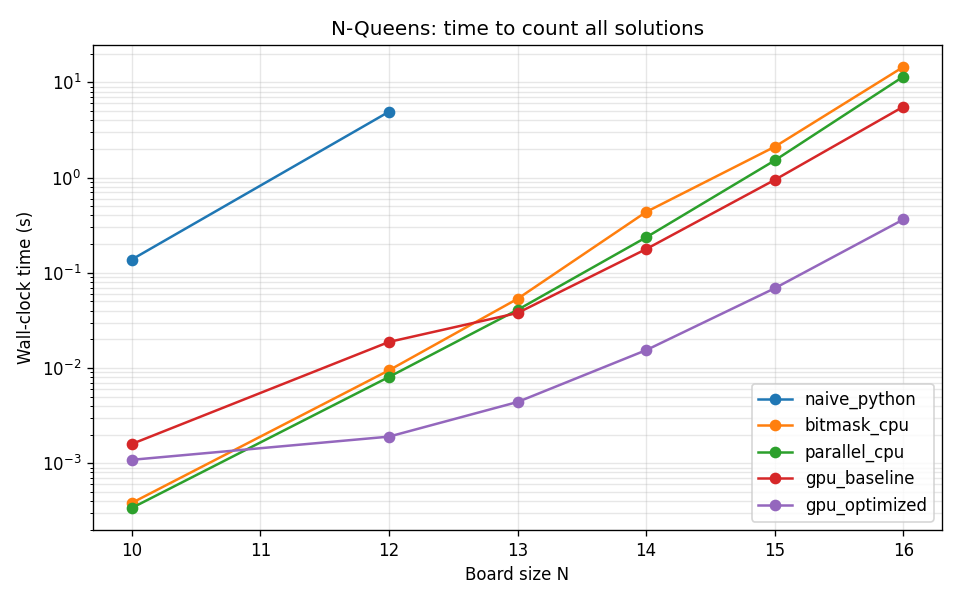
\includegraphics[width=\textwidth]{benchmarks.png}
    \caption{Wall-clock time vs.\ board size, log-y axis. All five implementations on the same axes; lower is better.}
    \label{fig:benchmarks}
\end{figure}

\subsection{Speedup vs.\ Bitmask CPU Baseline}

The bitmask CPU implementation is the appropriate baseline for speedup: it is the fastest \emph{single-threaded native} variant, isolating the contribution of parallelism from the contribution of native compilation. Table~\ref{tab:speedup} reports speedup relative to this baseline.

\begin{table}[H]
\centering
\caption{Speedup over Bitmask CPU (single-threaded native baseline). Values $< 1.0$ indicate a slowdown.}
\begin{tabular}{@{}rrrr@{}}
\toprule
$N$ & \textbf{Parallel CPU} & \textbf{GPU Baseline} & \textbf{GPU Optimised} \\
\midrule
10 & 1.13$\times$ & 0.24$\times$ & 0.35$\times$ \\
12 & 1.17$\times$ & 0.50$\times$ & 4.97$\times$ \\
13 & 1.31$\times$ & 1.41$\times$ & 12.13$\times$ \\
14 & 1.85$\times$ & 2.45$\times$ & 28.28$\times$ \\
15 & 1.39$\times$ & 2.23$\times$ & 30.63$\times$ \\
16 & 1.26$\times$ & 2.62$\times$ & \textbf{40.05$\times$} \\
\bottomrule
\end{tabular}
\label{tab:speedup}
\end{table}

\begin{figure}[H]
    \centering
    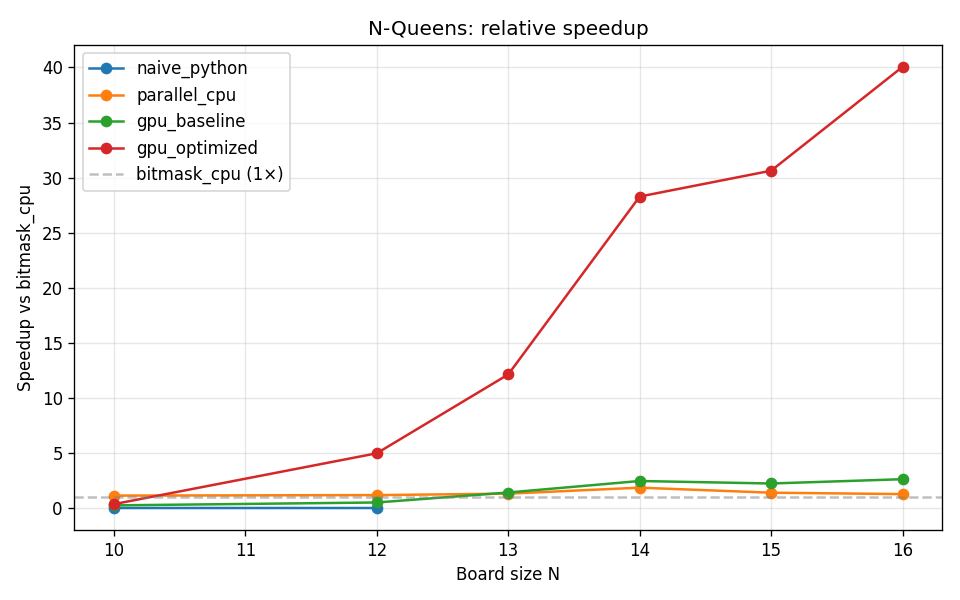
\includegraphics[width=\textwidth]{speedup.png}
    \caption{Speedup over Bitmask CPU. The GPU optimised variant pulls away after $N \geq 12$ and reaches 40$\times$ at $N = 16$.}
    \label{fig:speedup}
\end{figure}

\subsection{Key Observations}

\paragraph{JIT compilation alone gives ${\sim}500\times$.}
At $N = 12$, the naive Python recursion takes 4.91 s, while the bitmask Numba implementation takes 9.4 ms --- a 522$\times$ improvement. This is purely from native compilation and the bitmask trick; no parallelism is involved. It illustrates how much of the apparent ``parallel speedup'' in naive comparisons is in fact recovery from interpreter overhead.

\paragraph{Parallel CPU speedup is bounded by load imbalance.}
The Numba \texttt{prange} variant achieves only 1.13--1.85$\times$ over the serial bitmask baseline, far below the ideal scaling of the available vCPU count on Colab. This matches Quinn's prediction in \S 16.4: subtrees rooted at corner columns (e.g., $c_0 = 0$) prune quickly, while those rooted near the middle ($c_0 = N/2$) explore vastly more nodes. With static scheduling and 16 row-0 subtrees, several worker threads idle while the slowest worker continues.

\paragraph{GPU baseline is barely competitive at small $N$.}
At $N = 10$ and $N = 12$, GPU baseline is \emph{slower} than bitmask CPU (0.24$\times$ and 0.50$\times$ respectively). Two factors contribute: kernel launch and CUDA context overhead is in the millisecond range, dominating absolute times of $< 10$ ms; and the prefix count at $N = 10$ is only $\sim$70, leaving 97\% of the T4's 2{,}560 cores idle. The crossover where GPU baseline beats bitmask CPU occurs between $N = 12$ and $N = 13$, after which the speedup grows monotonically to 2.62$\times$ at $N = 16$.

\paragraph{GPU optimised dominates from $N \geq 12$.}
The optimised kernel reaches 40.05$\times$ over bitmask CPU at $N = 16$, and 15.30$\times$ over its own baseline (Table~\ref{tab:opt_decomp}). The deeper prefix lifts the thread count from $\sim$180 to $\sim$1{,}300 (an 8$\times$ increase in available parallelism); block-level reduction eliminates the per-thread global write of the baseline; and int32 masks halve register pressure. The combined effect is large enough that even at $N = 12$ the optimised GPU outperforms all CPU variants.

\paragraph{Crossover at small $N$ is unavoidable.}
At $N = 10$, all GPU variants underperform bitmask CPU. Any GPU implementation incurs a fixed cost (kernel launch, host-device synchronisation) that the CPU does not pay; below the crossover this cost exceeds the work itself. For practical N-Queens use, the GPU implementations are appropriate when the search exceeds $\sim$1 ms of CPU work, i.e. $N \geq 13$ in this configuration.

% ============================================================
\section{GPU Optimisation Analysis}
\label{sec:gpu_opt_analysis}

The optimised kernel applies three distinct optimisations on top of the baseline. This section dissects their individual contributions and the bottleneck each addresses.

\subsection{Optimisation 1 --- Deeper Prefix ($k=2 \to k=3$)}

The baseline partitions the search tree at depth 2, generating one CUDA thread per valid $(c_0, c_1)$ pair. For $N = 16$, this yields approximately $N(N-3) = 208$ valid prefixes. Even at full warp utilisation (32 threads per warp), this is only $\sim$7 active warps, against the T4's headline capacity of $40 \text{ SMs} \times 4 \text{ warps/SM} = 160$ concurrent warps.

The optimised variant partitions at depth 3. The valid $(c_0, c_1, c_2)$ triples obey four constraints (column distinctness, two adjacent-row diagonal checks, and one skip-row diagonal check $|c_2 - c_0| \neq 2$). For $N = 16$ this yields roughly 1{,}300 prefixes --- a 6.3$\times$ increase in available parallelism. The host-side enumeration cost is negligible ($O(N^3)$ pairs filtered by simple inequalities) and runs once per benchmark iteration.

\subsection{Optimisation 2 --- Block-Level Shared-Memory Reduction}

The baseline reduction strategy is per-thread: each thread writes its count to \texttt{out\_counts[tid]}, the host copies the array back, and \texttt{numpy.sum} reduces on the CPU. For $n_{\text{prefixes}}$ threads this costs $n_{\text{prefixes}}$ global memory writes plus $n_{\text{prefixes}} \times 8$ bytes of D2H transfer.

The optimised variant uses the standard CUDA parallel-reduction pattern. Each thread block of 128 threads cooperates to reduce its 128 per-thread counts in shared memory via a $\log_2 (128) = 7$-step tree, synchronised by \texttt{cuda.syncthreads()}. Thread 0 of each block then performs a single \texttt{cuda.atomic.add} into a one-element global counter. This reduces global memory writes by a factor of 128 (one atomic per block instead of one write per thread) and replaces the $n_{\text{prefixes}}$-element D2H copy with an 8-byte transfer.

\subsection{Optimisation 3 --- 32-bit Bitmasks}

The baseline uses \texttt{int64} for all bitmask state, despite all tested $N \leq 32$ fitting comfortably in 32 bits. The optimised variant uses \texttt{int32} throughout, halving the per-thread state size from $4 \times 32 \times 8 = 1024$ bytes (4 stacks $\times$ 32 entries $\times$ 8 bytes) to 512 bytes. Reduced register and local-memory pressure permits more concurrent thread blocks per SM, increasing achieved occupancy.

\subsection{Decomposition of the Speedup}

Table~\ref{tab:opt_decomp} compares the optimised kernel against its baseline for $N \geq 12$. The combined effect of the three optimisations grows from 9.87$\times$ at $N = 12$ to 15.30$\times$ at $N = 16$.

\begin{table}[H]
\centering
\caption{Speedup of GPU Optimised over GPU Baseline.}
\begin{tabular}{@{}rrrr@{}}
\toprule
$N$ & \textbf{Baseline (s)} & \textbf{Optimised (s)} & \textbf{Speedup} \\
\midrule
12 & 0.0188 & 0.0019 & 9.87$\times$ \\
13 & 0.0378 & 0.0044 & 8.61$\times$ \\
14 & 0.1774 & 0.0154 & 11.52$\times$ \\
15 & 0.9459 & 0.0688 & 13.75$\times$ \\
16 & 5.5547 & 0.3630 & \textbf{15.30$\times$} \\
\bottomrule
\end{tabular}
\label{tab:opt_decomp}
\end{table}

The trend is consistent: the optimisations scale with problem size, because all three target effects (occupancy, memory traffic, register pressure) compound as the kernel does more work per launch.

% ============================================================
\section{Correctness Validation}
\label{sec:correctness}

All five implementations are validated against the OEIS A000170 sequence~\cite{oeisA000170}. Each implementation is asserted to produce the exact published count at every benchmarked board size; a single mismatch aborts the run. The validation is integrated into the timing harness (a result is only entered into the benchmark dataframe if its \texttt{ok} flag is true).

\begin{table}[H]
\centering
\caption{Solution counts produced by each implementation, compared against OEIS A000170. All counts agree exactly.}
\begin{tabular}{@{}rrrrrrr@{}}
\toprule
$N$ & \textbf{OEIS} & \textbf{Naive} & \textbf{Bitmask} & \textbf{Parallel} & \textbf{GPU Base.} & \textbf{GPU Opt.} \\
\midrule
10 &        724 &        724 &        724 &        724 &        724 &        724 \\
12 &     14{,}200 &     14{,}200 &     14{,}200 &     14{,}200 &     14{,}200 &     14{,}200 \\
13 &     73{,}712 &        --- &     73{,}712 &     73{,}712 &     73{,}712 &     73{,}712 \\
14 &    365{,}596 &        --- &    365{,}596 &    365{,}596 &    365{,}596 &    365{,}596 \\
15 &  2{,}279{,}184 &        --- &  2{,}279{,}184 &  2{,}279{,}184 &  2{,}279{,}184 &  2{,}279{,}184 \\
16 & 14{,}772{,}512 &        --- & 14{,}772{,}512 & 14{,}772{,}512 & 14{,}772{,}512 & 14{,}772{,}512 \\
\bottomrule
\end{tabular}
\label{tab:correctness}
\end{table}

The solution count is an integer comparison, so no tolerance threshold is required: a single off-by-one in the bitmask shifts or stack management would corrupt millions of nodes and produce a wildly wrong total --- the OEIS oracle is therefore an extremely sharp correctness signal.

% ============================================================
\section{Conclusions}
\label{sec:conclusions}

This project implemented and benchmarked five variants of N-Queens solution counting on Google Colab with a Tesla T4 GPU, following the backtrack-search and parallel-backtrack methodology of Quinn Chapter 16~\cite{quinn2004}.

\subsection{Summary of Findings}

\begin{itemize}
    \item \textbf{GPU optimised dominates from $N \geq 12$.} Reaches 40$\times$ over the single-threaded native baseline at $N = 16$ (0.363 s vs.\ 14.54 s); 15.3$\times$ over its own baseline kernel.
    \item \textbf{Native compilation alone gives 522$\times$.} The single biggest gain in the entire pipeline is the move from interpreted Python to JIT-compiled bitmask code --- before any parallelism is added.
    \item \textbf{CPU parallelism delivers only 1.3$\times$.} Far below ideal scaling, consistent with the load imbalance Quinn predicts in \S 16.4. Static scheduling assigns whole row-0 subtrees to threads, but those subtrees are not equal size.
    \item \textbf{The naive GPU port is barely competitive.} The 2-row-prefix kernel underutilises the T4 (only $\sim$180 threads at $N = 16$) and is slower than CPU at $N \leq 12$. GPU acceleration of irregular search is not a free lunch; it requires explicit attention to thread count, occupancy, and memory traffic.
    \item \textbf{Three GPU optimisations compound to 15$\times$.} Deeper prefix (more threads), block-level reduction (less global traffic), and 32-bit masks (lower register pressure). Each addresses a distinct GPU bottleneck.
    \item \textbf{Crossover at $N = 12$--$13$.} Below this size, kernel launch and synchronisation overhead dominates; above it, GPU parallelism pays for itself with a steeply rising speedup.
\end{itemize}

\subsection{Broader Lesson}

Combinatorial search on GPUs is not a regular numerical workload, and treating it as one yields disappointing performance (the baseline kernel at $N = 12$ is slower than the CPU). Useful GPU acceleration requires explicit countermeasures against irregularity: deeper task partitioning to surface enough parallelism, careful reduction strategy to minimise global memory traffic, and tight per-thread state to enable high occupancy. Quinn's conceptual framework (\S 16.4 on parallel backtrack, the load-imbalance issue, the value of priority-queue-based dynamic load balancing in \S 16.7) translates directly to the GPU setting --- the mechanisms differ but the underlying performance issues are identical.

\newpage
\printbibliography

\end{document}
